\chapter{Fundamentals}\label{cap:fundamentals}

This chapter introduces the fundamental concepts that underpin this work. We begin with an overview of key machine learning topics relevant to our study, including computer vision architectures, multimodal large language models, image preprocessing methods, training strategies, and evaluation metrics. We then examine the main challenges and limitations associated with these approaches, situating them within the broader context of our research.

Finally, we summarize the core ideas discussed in this chapter and explain how they connect to the remainder of the thesis. Overall, this chapter provides the conceptual and technical foundation necessary to understand the methods and results presented in the subsequent chapters, particularly for readers who may not be familiar with the underlying principles of machine learning and computer vision.


\section{Computer vision architectures}

\section{Multimodal Large Language Models}
\subsection{CLIP}

Contrastive Language-Image Pre-training (CLIP), introduced by ~\citep{radford2021learning}, proposes a departure from traditional supervised computer vision by replacing fixed, manually annotated label sets with large-scale natural language supervision. Instead of training a model to predict one among a predefined list of categories, CLIP learns directly from approximately 400 million image-text pairs collected from the internet. The central intuition is that natural language offers a far richer and more flexible supervisory signal than curated taxonomies such as ImageNet classes. Text descriptions associated with images encode not only object names, but attributes, relationships, actions, and contextual cues. By leveraging this weak but abundant supervision at web scale, CLIP aims to learn visual representations that are inherently aligned with language and therefore more transferable across tasks and domains.

Technically, CLIP is composed of two neural networks trained jointly: an image encoder (either a modified ResNet or a Vision Transformer) and a Transformer-based text encoder (see Figure
\ref{fig:clip_architecture}). Each encoder maps its input into a latent vector space, and both outputs are projected into a shared multimodal embedding space where cosine similarity measures semantic alignment. Rather than generating captions or predicting words token by token, CLIP uses a contrastive objective: given a minibatch of $(N)$ image-text pairs, the model learns to identify the correct pairing among all $(N^2)$ possible combinations. The training objective maximizes similarity between matched pairs and minimizes similarity between mismatched ones using a symmetric cross-entropy loss over temperature-scaled cosine similarities. This formulation significantly improves training efficiency compared to generative captioning approaches and enables stable large-scale training from scratch without pre-initialization from supervised models.

\begin{figure*}[!ht]
\centering
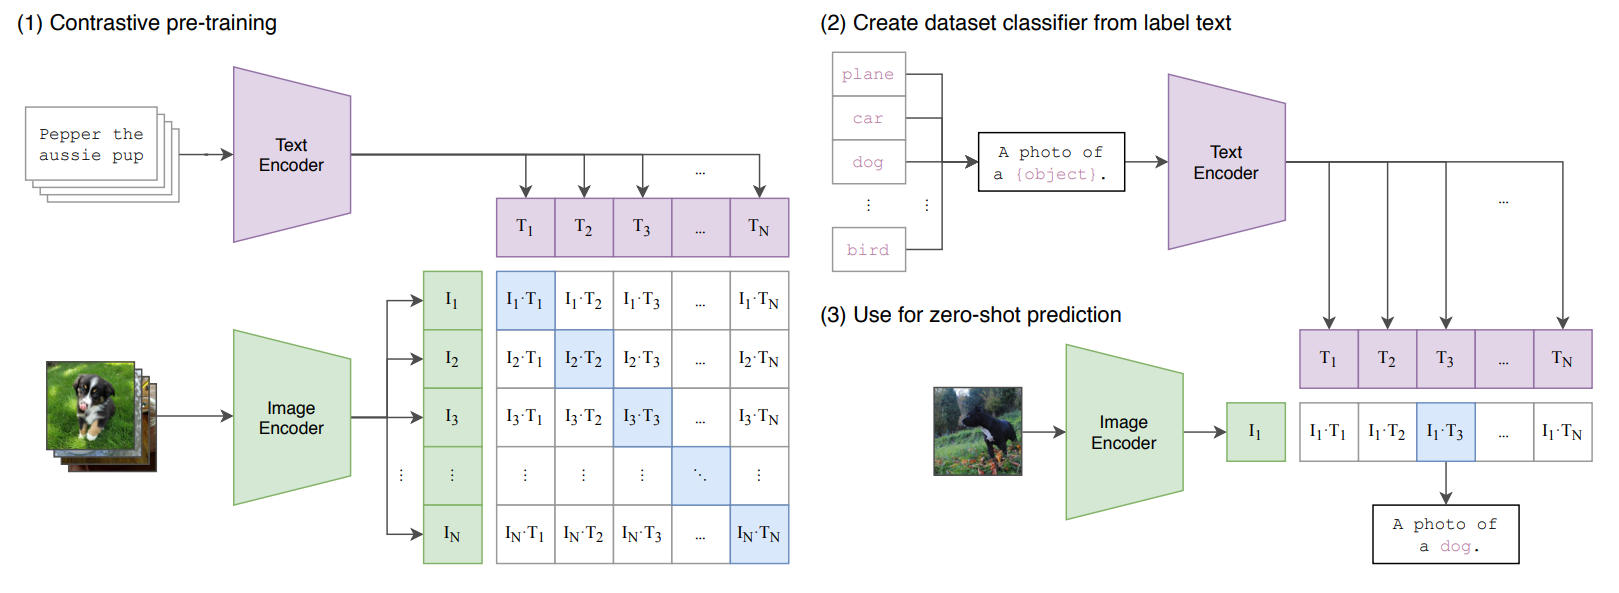
\includegraphics[width=6in]{images/clip.png}
\caption{CLIP architecture}
\legend{Source: \citet{radford2021learning}.}
\label{fig:clip_architecture}
\end{figure*}

A defining property of CLIP is its ability to perform zero-shot transfer. Because the model learns a joint embedding space aligned with natural language, it can be adapted to a new classification task without additional training. To classify images in a new dataset, one simply encodes textual prompts describing each class (e.g., “a photo of a dog”), embeds them using the text encoder, and compares them to image embeddings via cosine similarity . This effectively produces a linear classifier whose weights are dynamically generated from language. In zero-shot evaluation on ImageNet, CLIP achieves 76.2\% top-1 accuracy, matching the original supervised ResNet-50 despite using none of ImageNet's labeled training examples ~\citep{radford2021learning}. Across more than 30 datasets covering object recognition, fine-grained classification, action recognition, optical character recognition, and geo-localization, CLIP often performs competitively with fully supervised baselines, and in many cases surpasses linear probes trained on conventional ImageNet features.

Beyond raw performance, CLIP exhibits several notable empirical properties. Its zero-shot performance scales smoothly with model size and compute, following predictable log-log trends similar to those observed in large language models. Larger Vision Transformer variants outperform convolutional counterparts in compute efficiency, and representation learning evaluations show that CLIP features can exceed those of state-of-the-art supervised and self-supervised models on diverse benchmarks. At the same time, the model reveals limitations in tasks requiring fine spatial reasoning, counting, or highly specialized domain knowledge, highlighting that semantic alignment alone does not guarantee structured reasoning capabilities ~\citep{radford2021learning}. Overall, CLIP demonstrates that large-scale multimodal contrastive learning can produce open-vocabulary visual systems with strong generalization ability, establishing a foundation for subsequent multimodal and vision-language models.

\subsection{BLIP}
Bootstrapping Language-Image Pre-training (BLIP) is a vision–language framework designed to improve the performance of multimodal models on both understanding and generation tasks. Traditional vision–language models typically focus on a single category of tasks, such as image–text retrieval or image captioning. BLIP addresses this limitation by proposing a unified architecture capable of supporting a wide range of multimodal tasks. In addition to its architectural design, the framework introduces a data bootstrapping strategy that improves the quality of large-scale image–text datasets collected from the web, which often contain noisy or inaccurate captions ~\citep{li2022blip}. 

The BLIP model is built upon a Multimodal Mixture of Encoder–Decoder (MED) architecture that enables it to operate in multiple modes depending on the task being performed. The architecture combines a visual encoder, typically based on a Vision Transformer (ViT), with a text transformer that processes textual inputs and interacts with visual representations through cross-attention layers (see Figure
\ref{fig:blip_architecture}). This design allows the model to function as a unimodal encoder for representation learning, as an image-grounded text encoder for multimodal understanding, or as an image-grounded text decoder for text generation. As a result, BLIP can effectively learn relationships between visual content and language while also generating natural language descriptions conditioned on images  ~\citep{li2022blip}. 

\begin{figure*}[!ht]
\centering
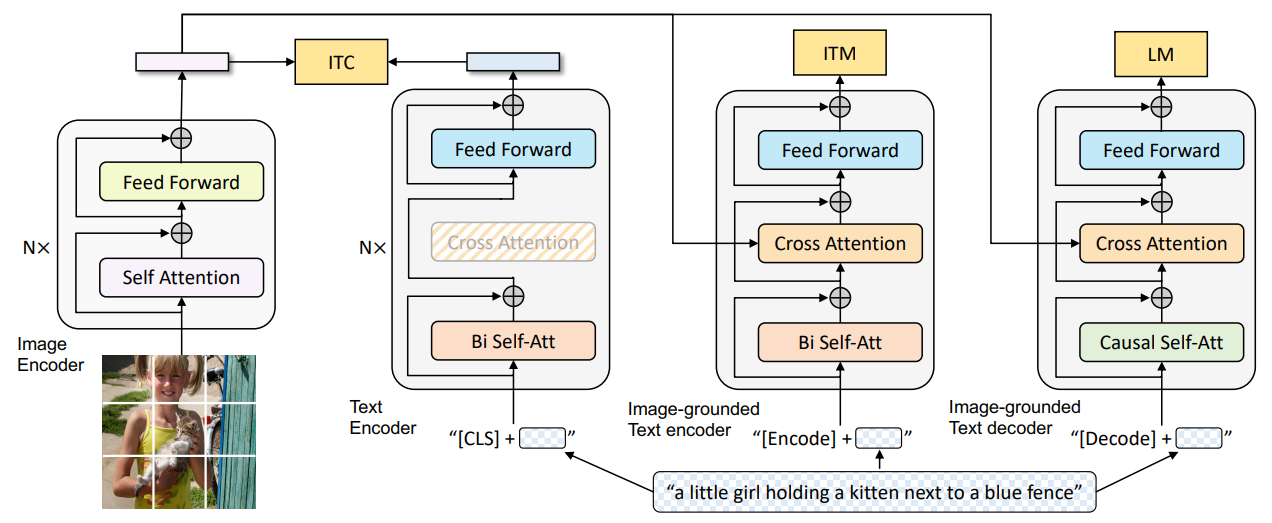
\includegraphics[width=6in]{images/blip.png}
\caption{BLIP architecture}
\legend{Source: \citet{li2022blip}.}
\label{fig:blip_architecture}
\end{figure*}

During pre-training, BLIP optimizes three complementary learning objectives that strengthen the alignment between images and text. The image–text contrastive (ITC) objective aligns visual and textual representations in a shared embedding space, improving retrieval performance. The image–text matching (ITM) objective determines whether a given image and text pair correspond to each other, encouraging the model to capture fine-grained multimodal relationships. Finally, a language modeling (LM) objective allows the model to generate textual descriptions from visual inputs using an autoregressive decoding process. Together, these objectives enable the model to perform both multimodal understanding and generation tasks within a single framework  ~\citep{li2022blip}. 

Another important contribution of BLIP is its Captioning and Filtering (CapFilt) data bootstrapping strategy, which improves the quality of training datasets. Web-collected image–text pairs often contain noisy captions that may not accurately describe the visual content. To address this issue, BLIP employs a captioning model to generate synthetic captions for images and a filtering model to remove low-quality text descriptions. This process produces a cleaner and more informative training dataset, which significantly enhances the model’s performance across several tasks, including image–text retrieval, image captioning, and visual question answering. Experimental results demonstrate that this approach leads to substantial improvements compared to previous vision–language models trained on similar data scales ~\citep{li2022blip}. 

\subsection{GPT}
The Generative Pre-trained Transformer (GPT) is a family of large language models designed to understand and generate natural language text. GPT models are based on the Transformer architecture and are trained using large-scale text corpora to learn statistical patterns in language. Through this training process, the model learns to predict the next token in a sequence given the previous context, enabling it to generate coherent and contextually relevant text. Because of this autoregressive formulation, GPT can perform a wide variety of language tasks without requiring task-specific architectures ~\citep{achiam2023gpt}. 

GPT models rely on a Transformer-based architecture that uses self-attention mechanisms to model relationships between tokens in a sequence. During training, the model processes large amounts of text data and learns representations that capture syntactic, semantic, and contextual information. The model is first trained through a large-scale pretraining phase using unlabeled text data and later refined through post-training techniques such as reinforcement learning with human feedback (RLHF), which aligns the model’s outputs with human preferences and improves instruction-following capabilities ~\citep{achiam2023gpt}. 

Due to their ability to generate and interpret language, GPT models can be applied to a broad range of natural language processing tasks. These include text generation, question answering, summarization, translation, code generation, and conversational agents. More recent versions of the model also support multimodal inputs and can interact with external tools and systems to perform more complex reasoning tasks. In practical applications, GPT models are frequently used in chatbots, educational tools, research assistance, and software development environments ~\citep{achiam2023gpt}. 

Experimental evaluations demonstrate that modern GPT models achieve strong performance across many academic and professional benchmarks (see Figure
\ref{fig:gpt_results}). For instance, GPT-4 has been shown to outperform previous language models on a wide range of tasks and achieve human-level performance on several standardized exams and professional assessments. Results reported in the study indicate that the model performs competitively across multiple domains, including science, mathematics, law, and general knowledge tests, highlighting the broad capabilities of large-scale language models ~\citep{achiam2023gpt}. 

\begin{figure*}[!ht]
\centering
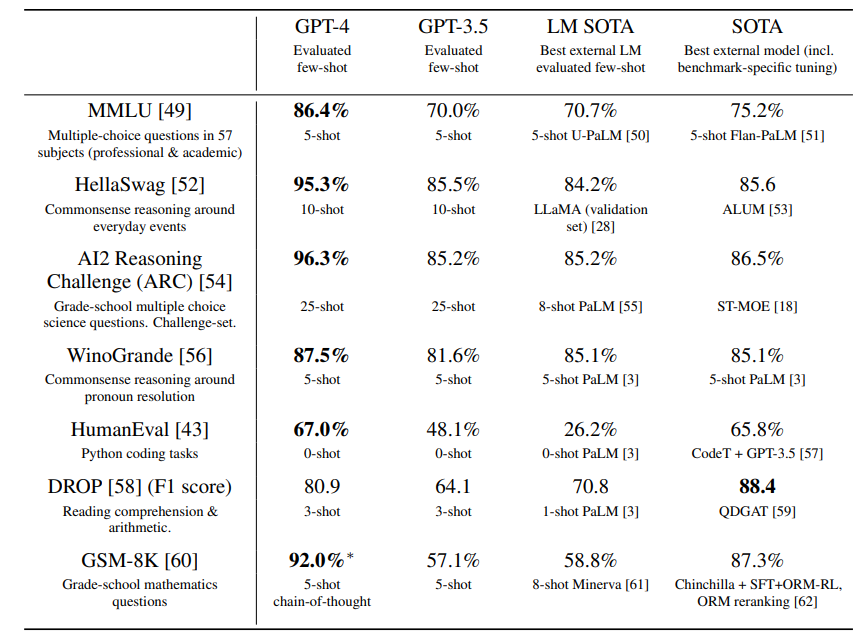
\includegraphics[width=6in]{images/gpt.png}
\caption{Performance of GPT-4 across multiple academic benchmarks as reported by the authors. The results show that GPT-4 consistently outperforms previous language models and achieves competitive performance compared with state-of-the-art systems trained specifically for individual benchmarks, demonstrating strong few-shot learning capabilities across diverse evaluation tasks.}
\legend{Source: \citet{achiam2023gpt}.}
\label{fig:gpt_results}
\end{figure*}

\subsection{Gemini}
Gemini is a family of large multimodal artificial intelligence models developed to advance capabilities in reasoning, language understanding, and cross-modal processing. Unlike traditional language models that primarily operate on text, Gemini was designed from the outset as a natively multimodal system, capable of processing and reasoning over multiple types of data, including text, images, audio, and video \citet{team2023gemini}. The model family includes different variants—Gemini Ultra, Gemini Pro, and Gemini Nano—which are optimized for different levels of computational capability and deployment environments. Ultra represents the most powerful model for complex reasoning and multimodal tasks, Pro is optimized for performance and efficiency across a wide range of applications, and Nano is designed for on-device deployment in resource-constrained environments. 

The architecture of Gemini is based on an enhanced decoder-only Transformer model, incorporating architectural improvements and optimization techniques to enable stable large-scale training. The models support long context windows of up to 32,000 tokens and use efficient attention mechanisms such as multi-query attention to improve computational efficiency. A key innovation of Gemini is its ability to process interleaved multimodal inputs, meaning that text, images, audio signals, and video frames can be provided within the same sequence of tokens (see Figure
\ref{fig:gemini_architecture}). Visual and video information are encoded as sequences of image frames within the context window, while audio signals are represented using features extracted from speech models. This design allows Gemini to perform complex reasoning tasks that require integrating information from multiple modalities within a single unified framework \citet{team2023gemini}. 

\begin{figure*}[!ht]
\centering
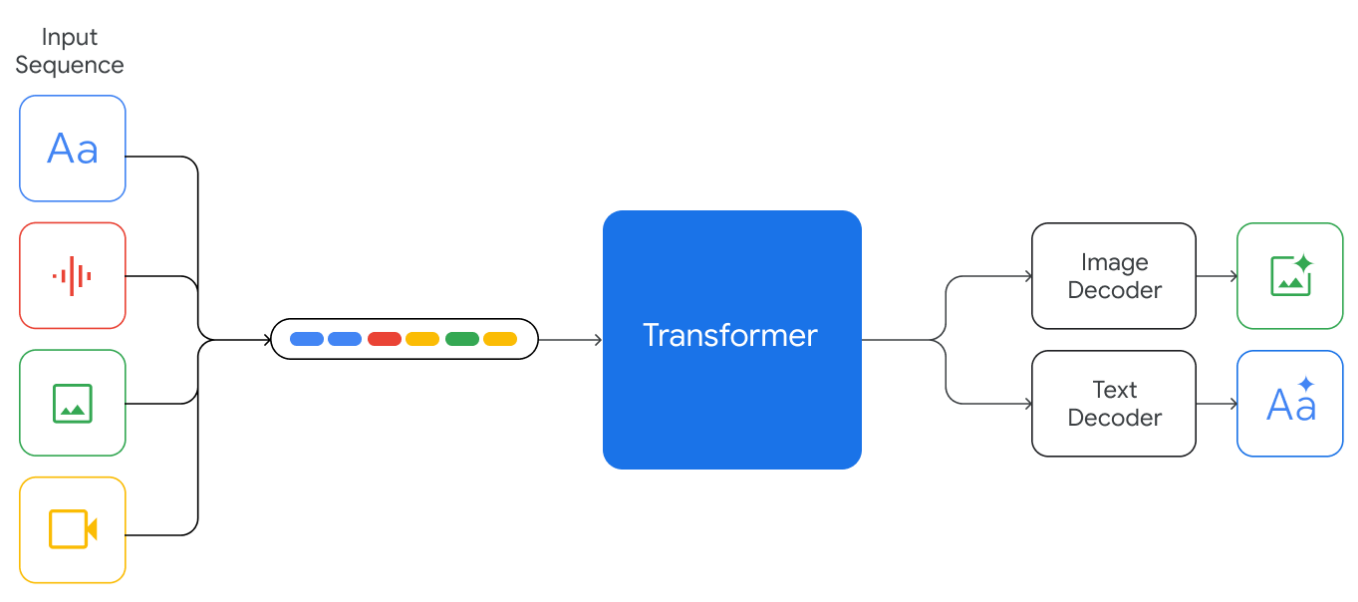
\includegraphics[width=6in]{images/gemini.png}
\caption{Illustration of the multimodal reasoning capabilities of Gemini models. According to the authors, Gemini can process sequences containing interleaved text, images, audio, and video, enabling the model to generate responses that combine textual and visual information within a unified multimodal framework}
\legend{Source: \citet{team2023gemini}.}
\label{fig:gemini_architecture}
\end{figure*}

Gemini models are trained on a large-scale multimodal and multilingual dataset composed of web documents, books, code repositories, images, audio, and video data. The training process involves extensive data filtering and safety mechanisms to ensure quality and remove harmful content. During pre-training, the model learns representations that capture relationships across different modalities, enabling it to perform tasks such as multimodal reasoning, content generation, summarization, and information extraction \citet{team2023gemini}. After pre-training, additional post-training procedures—including instruction tuning and reinforcement learning from human feedback—are applied to improve the model's ability to follow instructions and generate responses aligned with human expectations. 

Experimental results demonstrate that Gemini models achieve state-of-the-art performance across multiple benchmarks, including tasks involving reasoning, mathematics, coding, and multimodal understanding. In particular, Gemini Ultra surpasses human-expert performance on the MMLU benchmark, achieving an accuracy of approximately 90\%, and sets new state-of-the-art results across a wide range of text, image, audio, and video evaluation tasks. The model also shows strong performance in mathematical reasoning benchmarks such as GSM8K and coding benchmarks like HumanEval. These results highlight Gemini's ability to function as a general-purpose multimodal model capable of solving complex problems and enabling applications in areas such as education, software development, accessibility technologies, and intelligent assistants \citet{team2023gemini}.

\section{Image preprocessing techniques}
Image preprocessing is a fundamental step in computer vision pipelines, as raw images often need to be transformed into a standardized format before being used to train machine learning models. These preprocessing operations ensure that the data are compatible with the input requirements of neural network architectures and that the training process remains stable and efficient. Common preprocessing procedures include operations such as image resizing, normalization of pixel values, and data augmentation. Together, these techniques help prepare image datasets for effective learning by reducing variability caused by acquisition conditions while preserving relevant visual information.

One of the most common preprocessing steps is normalization, which consists of scaling the pixel intensity values to a standardized numerical range. Image pixel values are typically represented in the range ([0, 255]), and normalization transforms these values to smaller intervals such as ([0, 1]) or ([-1, 1]). In deep learning pipelines, it is also common to standardize images using the mean and standard deviation computed from the training dataset or from widely used datasets such as ImageNet. This procedure helps stabilize gradient updates during optimization and often accelerates the convergence of training algorithms by ensuring that input features have comparable numerical scales \citep{goodfellow2016deep}.

Another important preprocessing operation is image resizing, which adjusts the spatial resolution of images to match the input dimensions expected by the model architecture \citep{goodfellow2016deep}. Many convolutional neural networks require fixed-size inputs, such as (224 X 224) or (299 X 299) pixels, which makes resizing a necessary step when working with datasets containing images of varying resolutions. Resizing can be performed using interpolation techniques that preserve the overall structure of the visual content while adapting it to the required size. Although some modern architectures are capable of processing images with variable spatial dimensions, resizing remains widely used to standardize inputs and optimize computational efficiency during training and inference.

Data augmentation is another critical preprocessing technique that aims to artificially increase the diversity of the training dataset by applying controlled transformations to existing images (see Figure \ref{fig:data-augmentation}). These transformations may include horizontal or vertical flipping, rotations, random cropping, translations, and adjustments to color properties such as brightness, contrast, and saturation \citep{maharana2022review, shorten2019survey}. By exposing the model to multiple variations of the same image, data augmentation helps reduce overfitting and improves the ability of the model to generalize to unseen data. However, designing an effective augmentation pipeline can be challenging, as the choice of transformations and their parameters must be consistent with the characteristics of the dataset and the target task. Excessive or inappropriate transformations may distort relevant visual features or introduce unrealistic patterns, potentially degrading model performance. Consequently, careful selection and tuning of preprocessing strategies are essential to achieve robust and reliable results in computer vision applications \citep{maharana2022review}.

\begin{figure*}[!ht]
\centering
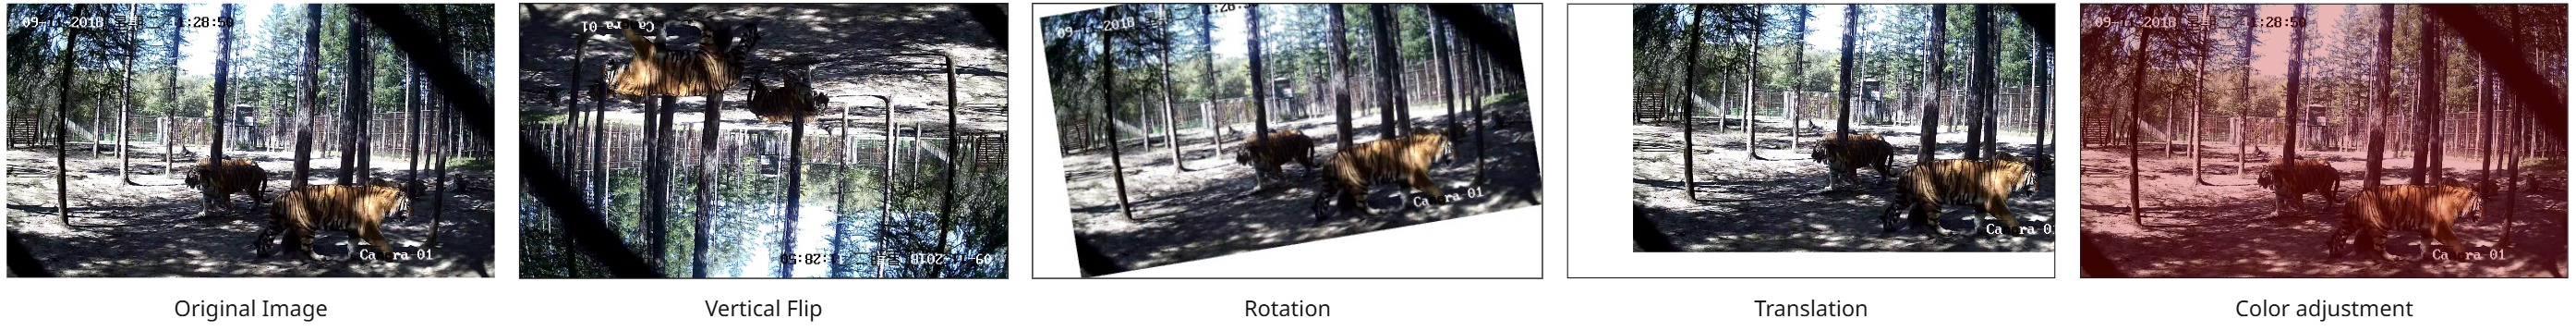
\includegraphics[width=6in]{images/data-augmentation.png}
\caption{Data augmentation examples}
\legend{Source: Author.}
\label{fig:data-augmentation}
\end{figure*}

\section{Training techniques}
The training of deep neural networks represents a high-dimensional, non-convex optimization problem where the objective is to minimize a loss function $\mathcal{L}(\theta)$ relative to a set of parameters $\theta \in \mathbb{R}^d$. This process is not merely a computational exercise in gradient descent but a complex interplay between algorithmic stability, numerical convergence, and the ultimate goal of statistical generalization \cite{goodfellow2016deep}.

\subsection{The Optimization Landscape: SGD vs. Adaptive Methods}

At the core of neural network training is the optimization landscape, a manifold characterized by saddle points, plateaus, and local minima. The choice of optimizer determines how the trajectory of $\theta$ navigates this surface.

\subsubsection{Stochastic Gradient Descent (SGD)}
SGD remains the foundational algorithm, updating parameters via:
\begin{equation}
\theta_{t+1} = \theta_t - \eta \nabla \mathcal{L}(\theta_t; x^{(i)}, y^{(i)})
\end{equation}
where $\eta$ is the learning rate. While computationally efficient, vanilla SGD often struggles with "ravines" where the surface curves much more steeply in one dimension than another. The introduction of momentum mitigates this by accumulating a velocity vector, effectively smoothing the path and accelerating convergence in consistent directions.

\subsubsection{Adaptive Methods: Adam and Beyond}
Adaptive optimizers, most notably Adam (Adaptive Moment Estimation), maintain per-parameter learning rates. Adam computes individual updates based on estimates of the first and second moments of the gradients:
\begin{align}
m_t &= \beta_1 m_{t-1} + (1 - \beta_1)g_t \\
v_t &= \beta_2 v_{t-1} + (1 - \beta_2)g_t^2
\end{align}
While Adam typically exhibits faster initial convergence, empirical evidence suggests that SGD with momentum often leads to better generalization on the test set \cite{wilson2018marginalvalueadaptivegradient}.

\subsection{Dynamic Training Protocols}

Optimization is rarely a static process. To navigate the loss surface effectively, researchers employ dynamic protocols that adjust the training regime in real-time.

\begin{itemize}
    \item \textbf{Learning Rate (LR) Scheduling:} A static $\eta$ is often suboptimal. Early training requires a high $\eta$ to escape local suboptimality, while later stages require a decaying $\eta$ to settle into the global minimum.
    \item \textbf{Early Stopping:} This serves as a temporal regularizer. By monitoring the loss on a disjoint validation set, training is halted once the validation error begins to diverge from the training error, preventing the model from memorizing noise.
\end{itemize}

\subsection{Regularization and the Bias-Variance Tradeoff}

The fundamental challenge in deep learning is the bias-variance tradeoff: balancing the model's ability to fit the training data against its ability to perform on unseen data.

\subsubsection{Weight Decay ($L_2$ Regularization)}
Weight decay modifies the objective function by adding a penalty term proportional to the square of the magnitude of the weights:
\begin{equation}
\mathcal{L}_{reg} = \mathcal{L} + \lambda \sum \theta^2
\end{equation}
This forces the optimization process to prefer smaller weights, resulting in a smoother mapping function.

\subsubsection{Dropout}
Dropout is a stochastic regularization technique where, during each training iteration, a fraction $p$ of neurons is randomly set to zero. This prevents co-adaptation, where neurons rely on the presence of specific other neurons to correct their errors \cite{srivastava2014dropout}.

\subsection{Practical Challenges and Modern Solutions}

\begin{itemize}
    \item \textbf{Vanishing and Exploding Gradients:} In deep networks, backpropagation can cause gradients to vanish or explode. Modern solutions include residual connections (ResNets) and gradient clipping.
    \item \textbf{Internal Covariate Shift:} As parameters change, the distribution of inputs to subsequent layers shifts. Batch Normalization (BN) addresses this by normalizing activations to have zero mean and unit variance within a mini-batch \cite{ioffe2015batch}.
\end{itemize}

\subsection{Mathematical Analysis of Adam's Convergence}

The convergence of Adam is analyzed through Regret Analysis. For a sequence of convex loss functions $f_1, \dots, f_T$, the regret $R(T)$ is bounded by:
\begin{equation}
R(T) = \sum_{t=1}^T [f_t(\theta_t) - f_t(\theta^*)] \leq O(\sqrt{T})
\end{equation}
However, it is critical to note that Adam can fail to converge in specific settings where the effective learning rate increases over time \cite{reddi2019convergenceadam}. The AMSGrad variant addresses this by ensuring $\hat{v}_t = \max(\hat{v}_{t-1}, v_t)$.

\section{Evaluation Metrics}

The rigorous assessment of model performance is a cornerstone of deep learning research. Relying on a single scalar value often fails to capture the nuances of model behavior, particularly in complex high-dimensional feature spaces. This section details the mathematical and conceptual frameworks for evaluating classification performance, with a specific focus on metrics robust to class distribution shifts.

\subsection{Classification Metrics}

Classification performance is typically derived from the \textit{Confusion Matrix}, which partitions predictions into True Positives ($TP$), True Negatives ($TN$), False Positives ($FP$), and False Negatives ($FN$). While these counts provide a raw view of performance, normalized metrics are required for comparative analysis.

\subsubsection{Accuracy}
Accuracy represents the ratio of correctly predicted observations to the total observations:
\begin{equation}
\text{Accuracy} = \frac{TP + TN}{TP + TN + FP + FN}
\end{equation}
Despite its ubiquity, accuracy is notoriously misleading in the presence of \textbf{class imbalance}. In a dataset where 99\% of samples belong to the majority class, a "naive" classifier that always predicts the majority class achieves 99\% accuracy while failing to learn any discriminative features of the minority class.

\subsubsection{Precision, Recall, and the F1-Score}
To address the limitations of accuracy, we employ metrics that isolate the performance on the positive (often minority) class:

\begin{itemize}
    \item \textbf{Precision (Positive Predictive Value):} Measures the fidelity of the model's positive predictions. It is the ratio of correctly predicted positive observations to the total predicted positives.
    \begin{equation}
    \text{Precision} = \frac{TP}{TP + FP}
    \end{equation}
    
    \item \textbf{Recall (Sensitivity):} Measures the model's ability to find all relevant cases within a dataset. 
    \begin{equation}
    \text{Recall} = \frac{TP}{TP + FN}
    \end{equation}
    
    \item \textbf{F1-Score:} The harmonic mean of Precision and Recall. Unlike the arithmetic mean, the harmonic mean penalizes extreme values, ensuring that a high F1-score requires both high precision and high recall.
    \begin{equation}
    F_1 = 2 \cdot \frac{\text{Precision} \cdot \text{Recall}}{\text{Precision} + \text{Recall}}
    \end{equation}
\end{itemize}

In doctoral research, the choice between these depends on the \textbf{cost of error}. In medical diagnosis, high Recall is often prioritized to avoid missing true cases (False Negatives), whereas in spam detection, high Precision is favored to avoid misclassifying legitimate emails (False Positives).

\subsection{Precision-Recall Curve}

In many deep learning architectures, the final layer outputs a probability distribution rather than a discrete label. The conversion to a label depends on a \textit{classification threshold} $\tau$ (conventionally set at 0.5). However, the optimal $\tau$ is rarely static.

\subsubsection{The Threshold Trade-off}
The Precision-Recall (PR) curve is constructed by plotting Precision against Recall at every possible threshold $\tau \in [0, 1]$. As the threshold decreases, the model becomes more "permissive" increasing Recall but typically decreasing Precision as more False Positives are introduced.



\subsubsection{Area Under the Precision-Recall Curve (AUPRC)}
The AUPRC (or Average Precision) provides a single-figure summary of the PR curve:
\begin{equation}
\text{AUPRC} = \sum_{n} (R_n - R_{n-1}) P_n
\end{equation}
where $P_n$ and $R_n$ are the precision and recall at the $n$-th threshold. 

\subsubsection{PR vs. ROC in Imbalanced Scenarios}
While the Receiver Operating Characteristic (ROC) curve is frequently used, it can present an overly optimistic view of model performance when the negative class is overwhelming. This is because the False Positive Rate ($FP / (FP+TN)$) remains small due to the large $TN$ denominator. The PR curve, by contrast, does not include $TN$ in its primary axes, making it a far more sensitive and honest indicator of performance for imbalanced tasks common in anomaly detection and rare-event prediction.

\section{Final Remarks}

This chapter established the theoretical and technical frameworks—ranging from foundational deep learning to multimodal systems such as CLIP, BLIP, and Gemini—necessary for robust wildlife classification. The transition from unimodal computer vision to vision-language models demonstrates how semantic alignment between text and imagery enhances model generalization. Furthermore, the analysis of optimization, regularization, and preprocessing highlights the importance of algorithmic stability when processing high-variance visual data from outdoor environments. The focus on evaluation metrics robust to class imbalance, specifically the Precision-Recall curve and AUPRC, directly addresses the statistical underrepresentation of rare species in camera trap datasets. These fundamentals provide the theoretical justification and practical tools for the research problem. Ultimately, the multimodal reasoning and training protocols described here inform the methodological choices in subsequent chapters, ensuring that the resulting species classification approaches are technically sound and optimized for automated biodiversity monitoring.